%  A simple AAU report template.
%  2015-05-08 v. 1.2.0
%  Copyright 2010-2015 by Jesper Kjær Nielsen <jkn@es.aau.dk>
%
%  This is free software: you can redistribute it and/or modify
%  it under the terms of the GNU General Public License as published by
%  the Free Software Foundation, either version 3 of the License, or
%  (at your option) any later version.
%
%  This is distributed in the hope that it will be useful,
%  but WITHOUT ANY WARRANTY; without even the implied warranty of
%  MERCHANTABILITY or FITNESS FOR A PARTICULAR PURPOSE.  See the
%  GNU General Public License for more details.
%
%  You can find the GNU General Public License at <http://www.gnu.org/licenses/>.
%
%  A simple AAU report template.
%  2015-05-08 v. 1.2.0
%  Copyright 2010-2015 by Jesper Kjær Nielsen <jkn@es.aau.dk>
%
%  This is free software: you can redistribute it and/or modify
%  it under the terms of the GNU General Public License as published by
%  the Free Software Foundation, either version 3 of the License, or
%  (at your option) any later version.
%
%  This is distributed in the hope that it will be useful,
%  but WITHOUT ANY WARRANTY; without even the implied warranty of
%  MERCHANTABILITY or FITNESS FOR A PARTICULAR PURPOSE.  See the
%  GNU General Public License for more details.
%
%  You can find the GNU General Public License at <http://www.gnu.org/licenses/>.
%
\documentclass[11pt,twoside,a4paper,openright]{report}
%%%%%%%%%%%%%%%%%%%%%%%%%%%%%%%%%%%%%%%%%%%%%%%%
% Language, Encoding and Fonts
% http://en.wikibooks.org/wiki/LaTeX/Internationalization
%%%%%%%%%%%%%%%%%%%%%%%%%%%%%%%%%%%%%%%%%%%%%%%%
% Select encoding of your inputs. Depends on
% your operating system and its default input
% encoding. Typically, you should use
%   Linux  : utf8 (most modern Linux distributions)
%            latin1
%   Windows: ansinew
%            latin1 (works in most cases)
%   Mac    : applemac
% Notice that you can manually change the input
% encoding of your files by selecting "save as"
% an select the desired input encoding.
\usepackage[utf8]{inputenc}
% Make latex understand and use the typographic
% rules of the language used in the document.
\usepackage{subfig}
\usepackage{capt-of}
\usepackage[danish,english]{babel}
% Use the palatino font
\usepackage[sc]{mathpazo}
\linespread{1.05}         % Palatino needs more leading (space between lines)
% Choose the font encoding
\usepackage[T1]{fontenc}
%%%%%%%%%%%%%%%%%%%%%%%%%%%%%%%%%%%%%%%%%%%%%%%%
% Graphics and Tables
% http://en.wikibooks.org/wiki/LaTeX/Importing_Graphics
% http://en.wikibooks.org/wiki/LaTeX/Tables
% http://en.wikibooks.org/wiki/LaTeX/Colors
%%%%%%%%%%%%%%%%%%%%%%%%%%%%%%%%%%%%%%%%%%%%%%%%
% load a colour package
\usepackage{xcolor}
\definecolor{aaublue}{RGB}{33,26,82}% dark blue
% The standard graphics inclusion package
\usepackage{graphicx}
% Set up how figure and table captions are displayed
\usepackage{caption}
\captionsetup{%
  font=footnotesize,% set font size to footnotesize
  labelfont=bf % bold label (e.g., Figure 3.2) font
}
% Make the standard latex tables look so much better
\usepackage{array,booktabs}
\usepackage{tabularx}
% Enable the use of frames around, e.g., theorems
% The framed package is used in the example environment
\usepackage{framed}

%%%%%%%%%%%%%%%%%%%%%%%%%%%%%%%%%%%%%%%%%%%%%%%%
% Mathematics
% http://en.wikibooks.org/wiki/LaTeX/Mathematics
%%%%%%%%%%%%%%%%%%%%%%%%%%%%%%%%%%%%%%%%%%%%%%%%
% Defines new environments such as equation,
% align and split
\usepackage{amsmath}
% Adds new math symbols
\usepackage{amssymb}
% Use theorems in your document
% The ntheorem package is also used for the example environment
% When using thmmarks, amsmath must be an option as well. Otherwise \eqref doesn't work anymore.
\usepackage[framed,amsmath,thmmarks]{ntheorem}

%%%%%%%%%%%%%%%%%%%%%%%%%%%%%%%%%%%%%%%%%%%%%%%%
% Page Layout
% http://en.wikibooks.org/wiki/LaTeX/Page_Layout
%%%%%%%%%%%%%%%%%%%%%%%%%%%%%%%%%%%%%%%%%%%%%%%%
% Change margins, papersize, etc of the document
\usepackage[
  inner=28mm,% left margin on an odd page
  outer=41mm,% right margin on an odd page
  ]{geometry}
% Modify how \chapter, \section, etc. look
% The titlesec package is very configureable
\usepackage{titlesec}
\titleformat{\chapter}[display]{\normalfont\huge\bfseries}{\chaptertitlename\ \thechapter}{20pt}{\Huge}
\titleformat*{\section}{\normalfont\Large\bfseries}
\titleformat*{\subsection}{\normalfont\large\bfseries}
\titleformat*{\subsubsection}{\normalfont\normalsize\bfseries}
%\titleformat*{\paragraph}{\normalfont\normalsize\bfseries}
%\titleformat*{\subparagraph}{\normalfont\normalsize\bfseries}

% Clear empty pages between chapters
\let\origdoublepage\cleardoublepage
\newcommand{\clearemptydoublepage}{%
  \clearpage
  {\pagestyle{empty}\origdoublepage}%
}
\let\cleardoublepage\clearemptydoublepage

% Change the headers and footers
\usepackage{fancyhdr}
\pagestyle{fancy}
\fancyhf{} %delete everything
\renewcommand{\headrulewidth}{0pt} %remove the horizontal line in the header
\fancyhead[RE]{\small\nouppercase\leftmark} %even page - chapter title
\fancyhead[LO]{\small\nouppercase\rightmark} %uneven page - section title
\fancyhead[LE,RO]{\thepage} %page number on all pages
% Do not stretch the content of a page. Instead,
% insert white space at the bottom of the page
\raggedbottom
% Enable arithmetics with length. Useful when
% typesetting the layout.
\usepackage{calc}

%%%%%%%%%%%%%%%%%%%%%%%%%%%%%%%%%%%%%%%%%%%%%%%%
% Bibliography
% http://en.wikibooks.org/wiki/LaTeX/Bibliography_Management
%%%%%%%%%%%%%%%%%%%%%%%%%%%%%%%%%%%%%%%%%%%%%%%%
\usepackage[backend=bibtex,
  bibencoding=utf8,sorting=none
  ]{biblatex}
\addbibresource{bib/mybib}

\usepackage{csquotes}

%%%%%%%%%%%%%%%%%%%%%%%%%%%%%%%%%%%%%%%%%%%%%%%%
% Our own stuff
%%%%%%%%%%%%%%%%%%%%%%%%%%%%%%%%%%%%%%%%%%%%%%%%
%needed for one table
\usepackage{multirow}
%needed for a different table
\newcolumntype{Y}{>{\centering\arraybackslash}X}

%needed for code listings
\usepackage{listings}
%sets the language globally to C
\lstset{language=C}
%code formating
\usepackage{adjustbox}
\usepackage{float}
%\usepackage[usenames,dvipsnames]{xcolor}

\definecolor{codegreen}{rgb}{0,0.6,0}
\definecolor{codegray}{rgb}{0.5,0.5,0.5}
\definecolor{codepurple}{rgb}{0.58,0,0.82}
\definecolor{backcolour}{rgb}{0.95,0.95,0.92}
\definecolor{keywordblue}{rgb}{0.1,0,1}

\lstdefinestyle{CStyle}{
    backgroundcolor=\color{backcolour},
    commentstyle=\color{codegreen},
    keywordstyle=\color{keywordblue},
    numberstyle=\tiny\color{codegray},
    stringstyle=\color{codepurple},
    basicstyle={\footnotesize\ttfamily},
    breakatwhitespace=true,
    breaklines=true,
    captionpos=t,
    keepspaces=true,
    numbers=left,
    numbersep=5pt,
    showspaces=false,
    showstringspaces=false,
    showtabs=false,
    tabsize=2,
    language=C
}
\lstset{style=CStyle}

%%%%%%%%%%%%%%%%%%%%%%%%%%%%%%%%%%%%%%%%%%%%%%%%
% Misc
%%%%%%%%%%%%%%%%%%%%%%%%%%%%%%%%%%%%%%%%%%%%%%%%
% Add bibliography and index to the table of
% contents
\usepackage[nottoc]{tocbibind}
% Add the command \pageref{LastPage} which refers to the
% page number of the last page
\usepackage{lastpage}
% Add todo notes in the margin of the document
\usepackage[
%  disable, %turn off todonotes
  colorinlistoftodos, %enable a coloured square in the list of todos
  textwidth=\marginparwidth, %set the width of the todonotes
  textsize=scriptsize, %size of the text in the todonotes
  ]{todonotes}

%%%%%%%%%%%%%%%%%%%%%%%%%%%%%%%%%%%%%%%%%%%%%%%%
% Hyperlinks
% http://en.wikibooks.org/wiki/LaTeX/Hyperlinks
%%%%%%%%%%%%%%%%%%%%%%%%%%%%%%%%%%%%%%%%%%%%%%%%
% Enable hyperlinks and insert info into the pdf
% file. Hypperref should be loaded as one of the
% last packages
\usepackage{hyperref}
\hypersetup{%
	%pdfpagelabels=true,%
	plainpages=false,%
	pdfauthor={Bucur, Busemann, Klein},%
	pdftitle={P3 project},%
	pdfsubject={Pathfinding, as used in Rescuing Robots},%
	bookmarksnumbered=true,%
	colorlinks=false,%
	citecolor=black,%
	filecolor=black,%
	linkcolor=black,% you should probably change this to black before printing
	urlcolor=black,%
	pdfstartview=FitH%
}
%%%%%%%%%%%%%%%%%%%%%%%%%%%%%%%%%%%%%%%%%%%%%%%%%%%%%%%%%%%%%%%%%%%%%%%%%%%%%%%%%%%%%%%%%%%%%%%%
%%%%%%%%%%%%%%%%%	OUR STUFF
\usepackage{nicefrac}
\newcommand*\mean[1]{\overline{#1}}

%%COLORS FOR COLORCODING FILES IN TODOS%%
\definecolor{titlepages}{RGB}{0,200,82}%
\definecolor{preface}{RGB}{200,82,0}%
\definecolor{01introduction}{RGB}{82,100,200}%
\definecolor{02problemDescription}{RGB}{100,50,200}%
\definecolor{03physicalSetup}{RGB}{255,20,200}%
\definecolor{04mathematicalModelling}{RGB}{10,200,200}%
\definecolor{05ExperimentsAndLabWork}{RGB}{200,200,200}%
\definecolor{06modelValidationAndPerformance}{RGB}{200,200,0}%
\definecolor{07controllerDesign}{RGB}{4,229,69}%
\definecolor{08controllerImplementation}{RGB}{169,220,90}%
\definecolor{09discussion}{RGB}{50,100,150}%
\definecolor{10conclusion}{RGB}{150,100,50}%
\definecolor{11dataAcquisition}{RGB}{50,100,50}%
% package inclusion and set up of the document
\input{setup/hyphenations.tex}%
\input{setup/macros.tex}% my new macros

\begin{document}
%frontmatter
\pagestyle{empty} %disable headers and footers
\pagenumbering{roman} %use roman page numbering in the frontmatter
\newcommand{\HRule}{\rule{\linewidth}{0.5 mm}}
\begin{titlepage}

\begin{center}
% Upper part of the page
\iflanguage{danish}{%
	\includegraphics[width=0.6\textwidth]{figures/aau_logo_da}
}{%
	\includegraphics[width=0.6\textwidth]{figures/aau_logo_en}
}\\[0.5cm]

\textsc{\Large P4}\\[0.6cm]

% Title
\HRule \\[0.8cm]
{ \Huge \bfseries  COOL TITLE}\\[0.4cm]

  \Large{ - EVEN COOLER SUBTITLE -
  % insert your subtitle here
  }
\todo{title}
\HRule \\[1.2cm]

% Author and supervisor
\begin{minipage}{0.49\textwidth}
\begin{flushleft} \large
\emph{Students:}\\
Daniel Frederik Busemann\\
Razvan-Vlad Bucur\\
Troels Ulstrup Klein\\
\end{flushleft}
\end{minipage}
\begin{minipage}{0.49\textwidth}
\begin{flushright} \large
\emph{Supervisors:} \\
Petar Durdevic Løhndorf\\
Simon Pedersen
\end{flushright}
\end{minipage}

\vfill

% Bottom of the page
{\large \today}



\end{center}

\end{titlepage}

%\input{sections/no_logo_frontpage.tex}
\thispagestyle{empty}
{\small
\strut\vfill % push the content to the bottom of the page
\noindent Copyright \copyright{} Aalborg University 2017\par
\vspace{0.2cm}
\noindent \LaTeX \: was used for typesetting this report,
MatLab and Simulink were used for designing and verifying the controller and
GitHub for collaborating as a group \cite{GitHub}.
}
\clearpage
\pdfbookmark[0]{English title page}{label:titlepage_en}
\aautitlepage{%
  \englishprojectinfo{
    %title
  }{%
    Control Theory%theme
  }{%
    Fall Semester 2017 %project period
  }{%
    ED4-1-F18 % project group
  }{%
    %list of group members
    Daniel Frederik Busemann\\ 
    Razvan-Vlad Bucur\\
    Troels Ulstrup Klein
  }{%
    %list of supervisors
    Petar Durdevic Løhndorf\\
    Simon Pedersen
  }{%
    1 % number of printed copies
  }{%
    \today % date of completion
  }%
}{%department and address
  \textbf{Electronics and Computer Engineering}\\
  Aalborg University\\
  \href{http://www.aau.dk}{http://www.aau.dk}
}{% the abstract
	Here should be an abstract
	but we didn't write a good one yet.
	
	Our end goal is to control the flow of water in a system 
	consisting of three pumps in parallel.
	
	A secondary goal is to achieve this with minimal power 
	consumption.
	
	To minimise power consumption, the relations described in 
	the affinity laws are used,
	specifically power being proportional to the cube of flow.
	
	Using more than one pump, we can effectively change the 
	impeller size online,
	by adding or subtracting one pump at a time.
	
}
	\todo{write and abstract}
\cleardoublepage
\cleardoublepage
\chapter*{Preface\markboth{Preface}{Preface}}\label{ch:preface}
\addcontentsline{toc}{chapter}{Preface}
This report was made by three students from Aalborg University Esbjerg attending
the 4th semester of the Electronics and Computer Engineering course.
From this point on,
every mention of \textbf{we}, \textbf{the group} or \textbf{the authors} refers to the three co-authors listed below.

All resources produced for this project can be found on the GitHub repository \cite{GitHub}.
Selected resources are also in the appendix.

\vspace{\baselineskip}\hfill Aalborg University, \today
\vfill\noindent

\begin{center}
\begin{minipage}[b]{0.45\textwidth}
 \centering
 \rule{\textwidth}{0.5pt}\\
  Daniel Frederik Busemann\\
 {\footnotesize <dbusem16@student.aau.dk>}
\end{minipage}
\hfill
\begin{minipage}[b]{0.45\textwidth}
 \vspace{20mm}
 \centering
 \rule{\textwidth}{0.5pt}
    Razvan-Vlad Bucur\\
 {\footnotesize <rbucur16@student.aau.dk>}
\end{minipage}
\hfill
%
\begin{minipage}[b]{0.45\textwidth}
 \vspace{20mm}
 \centering
 \rule{\textwidth}{0.5pt}\\
    Troels Ulstrup Klein\\
 {\footnotesize <tklein11@student.aau.dk>}
\end{minipage}
\end{center}

\pdfbookmark[0]{Contents}{label:contents}
\pagestyle{fancy} %enable headers and footers again
\tableofcontents
\cleardoublepage
%mainmatter
\pagenumbering{arabic} %use arabic page numbering in the mainmatter
\chapter*{List of Abbreviations}
\begin{tabular*}{\textwidth}{@{\extracolsep{\fill}} l  r }
	DAQ 	& Data acquisition board\\
	MFM 	& Magnetic flow meter\\
	DP		& $\Delta$Pressure (delta Pressure)\\
	
\end{tabular*}
\chapter{Introduction}\label{ch:introduction}
\todo[inline]{do we want a list of abbreviations?}

\subsection*{Reading Guide}
\todo{what is supposed to be in here? a short explanation of what knowledge each chapter conveys?}
\chapter{Problem Description}\label{ch:probdesc}

\section{Problem Description}
This project is about different mathematical modelling approaches for a system consisting mainly of three pumps.
The modelling will be used to develop a controller governing the total flow $Q_{tot}$.
The system was already fully functionally available in our university.
No alterations on the setup were possible to complete our project,
since the system was simultaneously used by two other groups.
As control inputs were available the individual speed of each pump $\omega P_{1,2,3}$ and the valve opening of one control valve $CV_1$.

Sensed outputs on this system are individual flow, individual differential pressure, pressure over $CV_1$ and individual power consumption ($P_el$).
Individual meaning separate for each pump.

A Piping and Instrumentations Diagram (P\&ID) of the system is available in Appendix \ref{app:overview}.


\section{Control Methods}
Based on the properties of a system two different approaches to controlling it can be applied.
Classical Control refers to the use of transfer functions
and generally full output feedback.
This is generally preferred for simpler systems,
mostly Single Input Single Output (SISO) systems,
because one transfer function is needed for all connections between each input and output.
A very common and simple control scheme for these systems is the PID control,
explained later in Chapter \ref{ch:controldesign}.
\cite{Franklin2014}

Multiple Input Multiple Output (MIMO) systems are often modelled and controlled using state-space
modelling, where all inputs are combined into one input vector
and the plant is described as a combination of three to four matrices.
In modern control this approach is commonly used in combination with full state feedback,
where instead of the output an intermediate product (the states) are used for full-state feedback.
Since we are not using this approach in our project no detailed explanation will be given in this report.


\section{Problem Delimitation}
Our system can be seen as a SISO, MIMO or something in between,
depending on what is to be controlled.
If only a single pump is considered and only the output flow to be controlled,
it is a SISO system.
Using multiple pumps and controlling for example Q and H would effectively make it a MIMO system.

In this project,
we decided to use the system as a SISO system,
controlling the total flow of all three pumps by regulating a single pump.
Primary goals are therefore:

\begin{itemize}
\item Creation of a dynamic model for one pump
\item Design of a PID controller for Q
\item Tuning of said PID controller 
\end{itemize}

In addition we also had some secondary goals,
which we deemed not necessary for successful completion of the project,
but nice extras.

\begin{itemize}
\item Creation of a static model for one pump
\item Creation of a static model for multiple pumps
\item Design of a controller for the flow, taking efficiency into account
\end{itemize}

The dynamic model will be useful to tune the PID controller,
and give us a deeper insight into the working of the pumps.
It would also make it possible to simulate and theoretically test different controller designs.


\subsection{Requirements}\label{sub:req}
To have a goal while tuning the PID controller,
we gave ourselves the following requirements.

\begin{itemize}
\item Maximum Overshoot $M_p = 0\%$
\item Steady-state error $e_{ss} \leq 1 \%$
\end{itemize}

We chose not to put a requirement on the settling time $t_s$,
because we could not initially estimate how the system would behave,
since we had no previous experience with pumps.
\chapter{Physical Setup}\label{ch:physsetup}
\section{Pumps}
\todo[color=03physicalSetup]{talk more about the pumps used, because the only reason we use them is: "they are present in the setup", e.g. we don't care why other pumps are not as good. [debatable]}
\subsection{Principle}
Centrifugal pumps are the most commonly used type of pump, due to its many advantages, simple construction, relative low 
cost, reliability and quiet operation.

When the pump is in operation, an increase in the fluid pressure from the pump's inlet to its outlet is created. This pressure 
difference drives the fluid further through the system.

The pump creates a pressure difference by transferring mechanical energy from the motor to the fluid through the impeller. The fluid 
flows from the inlet to the impeller center and out along its blades.
The centrifugal force increases the fluid velocity and consequently the kinetic energy is transformed to pressure. 

The blades of the rotating impeller transfer energy to the fluid by increasing velocity and pressure. The fluid is sucked into the 
impeller at the impeller eye and flows through the impeller channels formed by the blades between the shroud and hub.

The design of the impeller depends on the requirements for application, pressure and flow. The impeller is the primary component 
determining the pump performance. Pumps variants are often created only by modifying the impeller.
\todo[color=03physicalSetup]{maybe a bit repetitive, formatting could be improved }

Figure \ref{fig:pump_sections} represents the cross section and the transverse section of a centrifugal pump.
\newpage
\begin{figure}[h]
    \centering
    \subfloat[Cross Section]{{\includegraphics[width=0.4\linewidth]{figures/pump_cross_section.PNG}}}
    \qquad
    \hfill
    \subfloat[Transverse Section]{{\includegraphics[width=0.4\linewidth]{figures/pump_above_view.PNG}}}
    \caption{Centrifugal Pump}
    \label{fig:pump_sections}
\end{figure}

\subsection{Affinity Laws}
Affinity laws are mathematical relationships that provide a way to estimate the changes in performance of a pump, as a result
of a change in one of the basic pump variables.
In it's simplest form, the term law, means a principle that has been proven true for all cases.
\todo[color=03physicalSetup]{add affinity laws, formula and statement}
\todo[color=03physicalSetup]{"proven true for all cases"? that can't be correct for an estimate}

\begin{equation}
	\left(\frac{N_1}{N_2}\right)^1 = \frac{Q_1}{Q_2}$$
	
	$$\left(\frac{N_1}{N_2}\right)^2 = \frac{H_1}{H_2}$$
	
	$$\left(\frac{N_1}{N_2}\right)^3 = \frac{P_1}{P_2}	
\end{equation} Equations for constant impeller diameter $D$ \cite{AffinityLaws}

\begin{equation}
	\left(\frac{D_1}{D_2}\right)^1 = \frac{Q_1}{Q_2}$$
	
	$$\left(\frac{D_1}{D_2}\right)^2 = \frac{H_1}{H_2}$$
	
	$$\left(\frac{D_1}{D_2}\right)^3 = \frac{P_1}{P_2}	
\end{equation} Equations for constant rotational speed $N$ \cite{AffinityLaws}


\subsection{Performance Curves}

\section{Pipes}
Pipes are a way of transporting liquids or gasses, inside a controllable environment.
They are used to interconnect the pumps and the tank and other peripherals.
One common analogy compares them to wires in electrical circuits.

Based on their diameters, material and shape,
they introduce resistance to the flow of the pumped medium.
Staying with the analogy to electrical circuits,
this can be compared to the cross sectional area and the specific resistance of a wire material.

\section{Valves}
Valves can control the resistance introduced, by changing the diameter of the pipeline at a given point. \todo[color=03physicalSetup]{re-write valves, this reads terrible}

The valve built into the used system is not used for control purposes,
but only to simulate disturbances downstream the pumps.

Depending on the type of valves, they can block the flow partially or completely.
Their reaction and settling time may change and their ability to withstand pressure.
Some valves have an inbuilt controller, managing the opening percentage.
Valves can be actuated by different means, for example air pressure, electric motors or handles
\todo[color=03physicalSetup]{there is a better word for handle in this context}

\section{Sensors}
To be able to monitor the system closely, different sensors are used.
\todo[color=03physicalSetup]{write about the sensors used in the system}

\subsection{Flow Meter}
\subsection{$\Delta$Pressure Sensor}
\subsection{Power Sensor}
\todo[color=03physicalSetup]{complete this list of subsections}
\todo[color=03physicalSetup]{maybe take out of ToC? (subsection*)}

\todo[color=03physicalSetup]{Do we want a section about xPC and Simulink Realtime?}

\chapter{Mathematical Modelling}\label{ch:mathmodel}

\section{Pump Curves}\label{sec:pumpcurves}


We decided to use the data gathered through experiments, to develop a model that would fit all our data within a small degree of error, 
and that we would be able to further test.

We decided to use black-box modeling with polynomial fitting. We based our decision on other research that has been done on the same
setup as ours, but also on trial and error.

Curve Fitting Tool \cite{cftool} \textit{cftool} was used in order to find a suitable mathematical formula for accurately describing the 
system, while also trying to represent it in the easiest manner possible. 

Equation \ref{eq:simulated_power} determines the power consumption, given the head and the flow. Although the formula does not directly
relate to the pump speed, it indirectly relates to it, due to the fact that only one possible pump speed $\omega$ exists for a given
pressure and flow.
\todo[color=04mathematicalModelling]{quote zhenyu paper maybe}
\begin{multline}
		P(Q,H) = p_{00} + p_{10} \cdot Q + p_{01} \cdot H + p_{20} \cdot Q^2 + p_{11} \cdot Q \cdot H + \\
		p_{02} \cdot H^2 + p_{30} \cdot Q ^ 3 + p_{21} \cdot Q^2 \cdot H + p_{12} \cdot Q \cdot H^2
		\label{eq:simulated_power}
\end{multline}
\todo[color=04mathematicalModelling]{maybe align formula}

The model has an adjusted coefficient of determination  $\bar{R^2}$ = 1. Such a high coefficient of determination, was achieved due to
heavy filtering of the data gathered. In addition, no or minor disturbances were present during the gathering of the data.
\todo[color=04mathematicalModelling]{from supervisor meeting} 


\newpage
With the data gathered through the experiments (Section \ref{sec:experiment}\todo[color=04mathematicalModelling]{not linked yet}),

\todo[color=04mathematicalModelling]{re-write this section, all math used here doesn't apply to real life. But use the knowledge we 
gained here instead of deleting everything}
We decided to use black-box modelling with polynomial fitting.
For this we used the Curve Fitting Tool \cite{cftool} \textit{cftool} 
\todo[color=04mathematicalModelling]{make this look like a command} in MATLAB.
Looking at the data we decided to use polynomial fitting with a second degree polynomial
as can be seen in equation \ref{eq:polynom}.

\begin{equation}
	 P(Q) = p_1 \cdot Q^2 + p_2 \cdot Q + p_3
	 \label{eq:polynom}
\end{equation}

After repeating this process over different datasets with different pump speeds,
we noticed that the coefficients $p_1$ and $p_2$ barely change.
\todo[color=04mathematicalModelling]{they do, shit isn't even properly linear...}

The standard deviation for the $p_1$ and $p_2$ coefficients were calculated with the equation \todo[color=04mathematicalModelling]{add 
reference to eq}

\begin{equation}
	\sigma_{\mean{p_{1,2}}} = \dfrac{1}{n}\sum |p_{1,2}-\mean{p_{1,2}}|
	\label{eq:avedev}
\end{equation}

The results obviously vary between runs. For the run used to create the model the $\sigma_{\mean{p_{1,2}}}$ are:
\begin{equation}
	\sigma_{\mean{p_1}} \simeq 0.003854$$
	
	$$\sigma_{\mean{p_2}} \simeq 0.042299
\end{equation}

The $p_3$ coefficient however changes significantly, through different pump speeds.
With a standard deviation $\sigma_{\mean{p_3}} \simeq 3.378111$ it was impossible to use only one simple polynomial as described in 
\ref{eq:polynom} to describe all pump characteristics at all speeds.

We were able to identify a second order polynomial describing the change in $p_3$ according to the pump speed $\omega$.
\begin{equation}
	 p_3 = a \cdot \omega^2 + b \cdot \omega + c
	 \label{eq:p3olynom}
\end{equation}

Combining \ref{eq:polynom} and \ref{eq:p3olynom}, we get:

\begin{equation}
	P(Q) = p_1 \cdot Q^2 + p_2 \cdot Q + a \cdot \omega^2 + b \cdot \omega + c 
\end{equation}
\todo[color=04mathematicalModelling]{at least something that isn't completely wrong, but incomplete. Not sure if we should start 
remodelling with power anyways}

\chapter{Experiments and Lab Work}\label{ch:experiment} 
\section{Performance test}\label{sec:performance_test} 
For gathering data about the pump system, a performance test was carried out.
\todo{Should we explain how a performance test is carried out?}
\todo{yes -Daniel wait, we do later, no?}

Instead of relying on performance curves provided by the pump manufacturer,
the pump will be run in situ \todo{"situ"? I think something went missing here}, and the obtained data will show how the pump 
operates for the specific system.
 
During the test flow resistance is varied by a choke valve, resulting in 
corresponding values of flow, differential pressure, and power consumption 
which has been measured in order to create the performance curves.
\newline
\newline
The programming for the pump test was done in Matlab. 
A model of the system was made using Simulink blocks. \todo{elaborate on this?}
Simulink Real-time and xPC Target was used to run the model in real-time 
on the pump systems dedicated PC. 
\todo{move somewhere else?} 

\missingfigure[figwidth=0.5\textwidth]{Placeholder figure}

xPC Target allows you to add I/O blocks to your model, and then use the host 
PC and a C compiler to create executable code. The executable code is download 
from the host PC to the target PC running the xPC Target real-time kernel. 
After downloading the executable code, you can run and test your target 
application in real-time. \todo{is it nescesarry to describe this and data acquisition?}

\missingfigure[figwidth=0.5\textwidth]{Placeholder figure}

\textbf{Experiment setup}
%- pumpspeeds to iterate through: 0:10:100\n
- time intervals from valve settling time, steps of 10 seconds
- select valve opening(backpressure) by for loop


- Results
\todo{Do we need the datasheet for the pump? We must be using it for something?? (NPSHR?)}
 
\chapter{Model Validation}\label{ch:modValPerf}
\section{Static Modelling}
\todo[color=06modelValidationAndPerformance]{Model Validation and Performance}
To validate the model acquired in Chapter \ref{ch:mathmodel}, we ran a second test with the 
same setup as described in Chapter \ref{ch:experiment}. Coefficients were determined for pump models,
for every percentage of the valve opening.

Equation \ref{eq:pumpHeadModel60} and \ref{eq:pumpPowerModel60} represent the modeled Flow and Power 
Consumption for 60 \% pump speed.

\begin{equation}
	H(\omega) = \frac{\bar{a_0}}{\bar{\omega_0^2}} \cdot \omega^2 + \frac{\bar{a_1}}{\bar{\omega_0}} \cdot \omega \cdot Q(\omega) + \bar{a_2} \cdot Q(\omega)^2
	\label{eq:pumpHeadModel60}
\end{equation}
\begin{equation}
	P(\omega) = \frac{\bar{b_0}}{\bar{\omega_0^3}} \cdot \omega^3 + \frac{\bar{b_1}}{\bar{\omega_0^2}} \cdot \omega^2 \cdot Q(\omega) + \frac{\bar{b_2}}{\omega_0} \cdot \omega \cdot Q(\omega)^2 + b_3 \cdot Q(\omega)^3
	\label{eq:pumpPowerModel60}
\end{equation}

The coefficients for the model were determined at 60 \% pump speed and can be seen below.

\begin{align*}
	\bar{a_0} = -0.03044 && \bar{a_1} = 0.07635  && \bar{a_2} = 1.688  \\
	\bar{b_0} = -0.2825 && \bar{b_1} = -0.7147 && \bar{b_2} = 54.39 && \bar{b_3} = 163.7 \\
	\bar{\omega_0} = 2298 rpm \\
\end{align*}
\newpage
Figures \ref{fig:flowVsModeledPressure} and \ref{fig:flowVsModeledPower}, represent the Pressure and 
the Power Consumption for one of the tests.

\begin{figure}[ht]
	\centering
	\includegraphics[width=0.8\textwidth]{figures/06ModelValidation/flowVsModeledPowerConsumption.eps}
	\caption{Flow Vs. Modeled Power Consumption}
	\label{fig:flowVsModeledPower}
\end{figure}
\begin{figure}[ht]
	\centering
	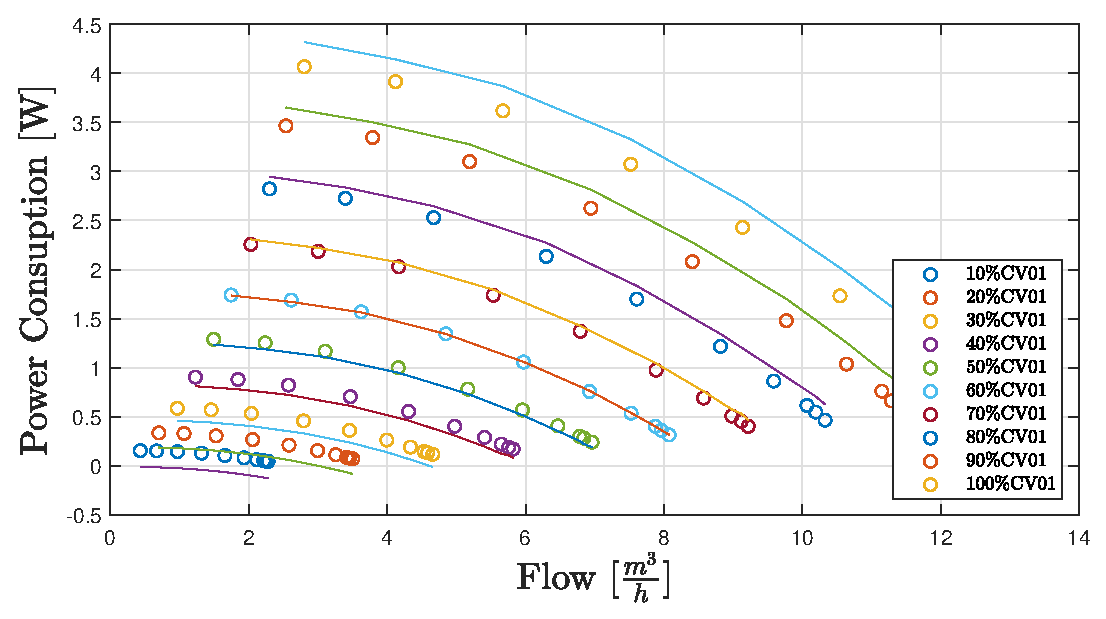
\includegraphics[width=0.8\textwidth]{figures/06ModelValidation/flowVsModeledPressure.eps}
	\caption{Flow Vs. Modeled Pressure}
	\label{fig:flowVsModeledPressure}
\end{figure}

As expected, the models are able to approximate the pump curves, that are closer to the actual pump speed 
the models were determined for. They are not as accurate overall as expected. 
The modelling errors could come as a result of many factors, however, there is room for improvement. 
As with the case of the pressure sensors, we were not able to determine accurate values for 
the pump speeds. Again, we have used gains and offsets provided to us. Additionally, as stated in \cite{Yang2010}
motor and drive efficiency are not accounted for.

\section{Dynamic Modelling}
We determined the coefficients for our P, I, and D using Ziegler Nichols tuning method.
The results both in theory and practice can be seen below. Figure \ref{fig:modeledPI2} represents the model for the PI -
Controller, while Figure \ref{fig:actualPI2} represents the output of the system using the same controller.

\begin{figure}[H]
	\centering
	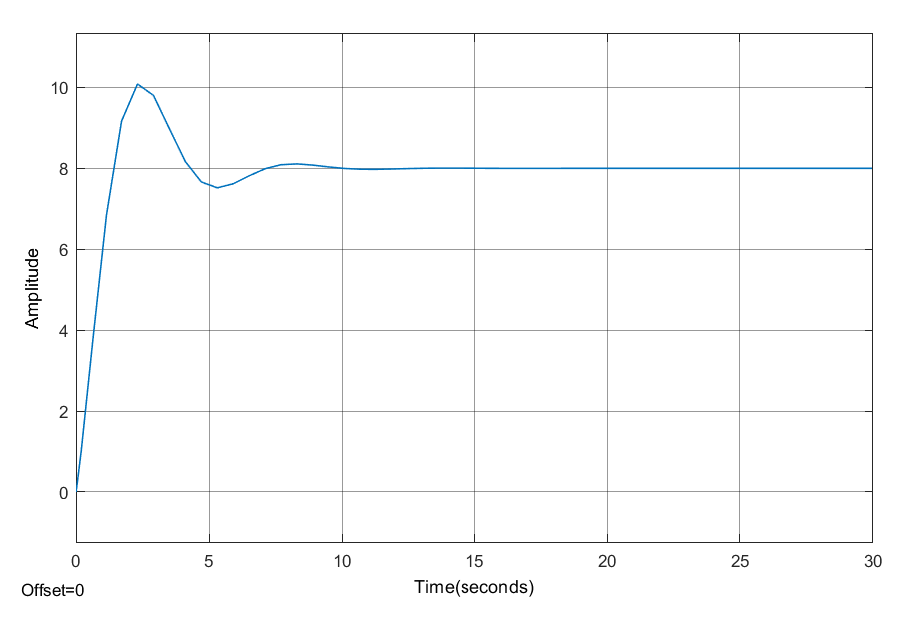
\includegraphics[width=0.7\textwidth]{figures/06ModelValidation/modelPI.eps}
	\caption{Modeled PI Controller}
	\label{fig:modeledPI2}
\end{figure}
\vspace{-5mm}
\begin{figure}[H]
    \centering
    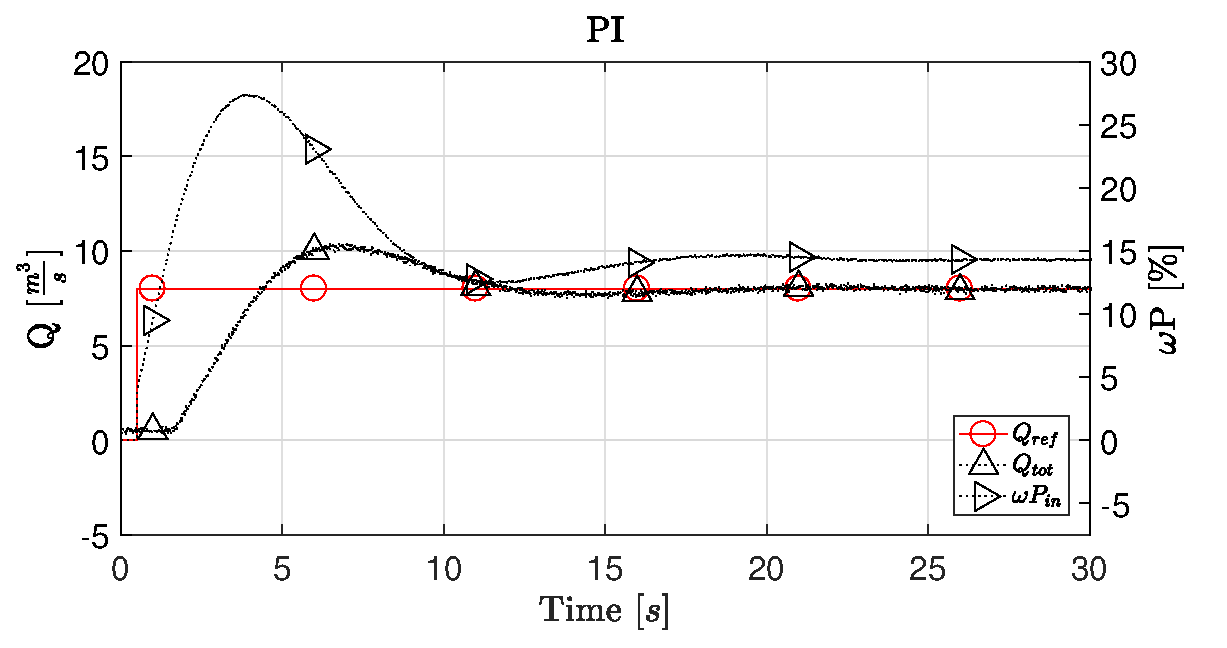
\includegraphics[width=\textwidth]{figures/07controllerDesign/PItest.eps}
    \caption{Actual PI Controller}
	\label{fig:actualPI2}
\end{figure}
The output of the model is quite similar to the output of the setup, with the exception of the delayed step input.
Additionally, the model seems to converge faster to the setpoint.

The model for the PID - Controller also presents strong similarities with the actual output of the setup.
The comparison can be seen in figures \ref{fig:modeledPID2} and \ref{fig:actualPID2}.
\begin{figure}[H]
	\centering
	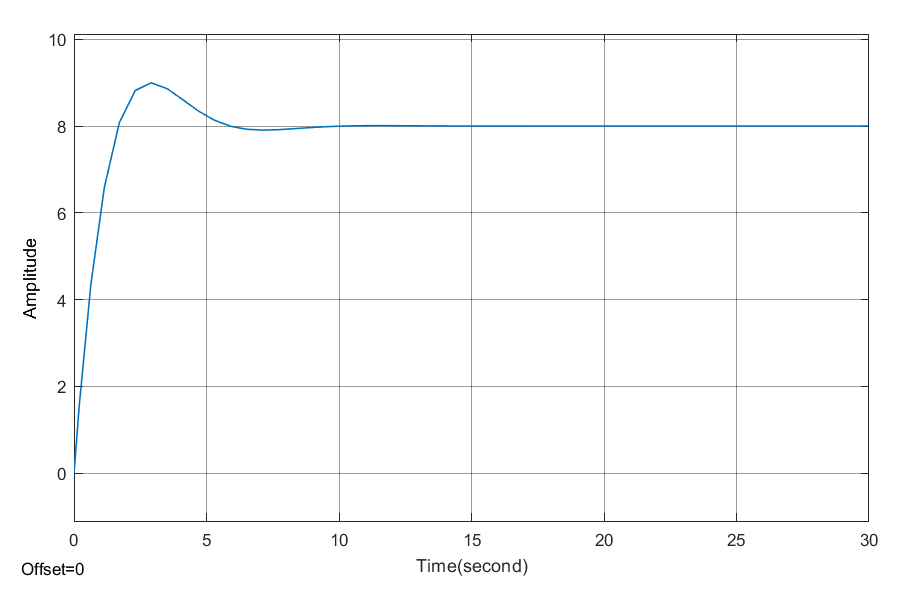
\includegraphics[width=0.7\textwidth]{figures/06ModelValidation/modelPID.eps}
	\caption{Modeled PID Controller}
	\label{fig:modeledPID2}
\end{figure}
\vspace{-5mm}
\begin{figure}[H]
    \centering
    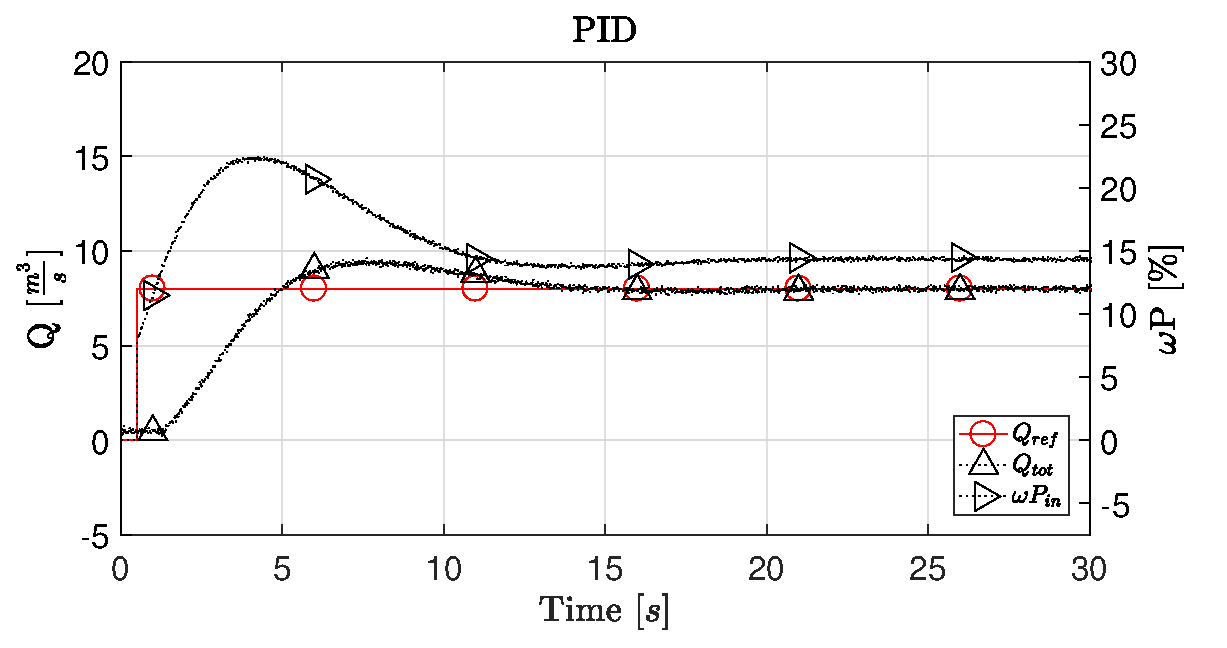
\includegraphics[width=\textwidth]{figures/07controllerDesign/PIDtest.eps}
    \caption{Actual PID Controller}
	\label{fig:actualPID2}
\end{figure}
Same can be noticed for the PID - Controller, the step input for the physical setup is given 0.5 seconds later.
The model also converges faster to the setpoint. This might be due to dynamic properties of the flow, 
which might not be properly modeled using the transfer function.
All figures can be found in Appendix  \ref{app:modelValidation}.
\chapter{Controller Design}\label{ch:controldesign}
\todo[color=07controllerDesign]{Controller Design not enough text yet}
\todo[color=07controllerDesign]{Explain what PID is}
\section{Step response}
\begin{figure}[H]
    \centering
    \includegraphics[width=0.75\textwidth]{figures/04ExperimentsAndLabWork/CLblock.pdf}
    \caption{A simplified block diagram to show the placement of a PID}
	\label{fig:PIDplace}
\end{figure}

For the common PID-tuning method as described by Ziegler and Nichols,
some knowledge about the system is needed.
There exist two Ziegler Nichols methods,
depending on the open-loop dynamics of the system.
Because our system has a stable response to a step input, we used the first method described in \todo[color=07controllerDesign]{page 226 ff, Feedback Control of Dynamic Systems}
Here typically a unit step input is given into the OL system as shown in figure \ref{fig:OL}.

\todo[color=07controllerDesign]{get actual values for R and L}
\begin{figure}[H]
    \centering
    \includegraphics[width=0.75\textwidth]{figures/04ExperimentsAndLabWork/OLblock.pdf}
    \caption{OL block diagram of the system}
\label{fig:OL}
\end{figure}

Because we are scaling the $\omega$ down by a factor of 10, so we can directly read the percentage,
we had to scale the aforementioned unit step up by a factor of 10,
in order to get usable results.
While encountering this problem, we also noticed, that the pumps don't spin below an $\omega$ of 9\%.
When using the corrected step input, we got the measurements shown in figure X \ref{fig:stepin}.

Our analysis of figure \ref{fig:stepin} gives us the following values:
\\
\begin{tabular}{r c l l}
	$A$ 	& $=$ & $2.2177$ 	& \footnotesize{\textit{final value}}\\
	$R$ 	& $=$ & $1.7833$ 	& \footnotesize{\textit{slope}}\\
	$t_d=L$	& $=$ & $0.75$ 		& \footnotesize{\textit{lag}}\\
	$\tau$ 	& $=$ & $1.2436$ 	& \footnotesize{\textit{time constant}}
\end{tabular}
\\
Ziegler-Nichols is tuning a PID controller $D_c(s)$ with the formula\\
$D_c(s)=k_P(1+ \frac{1}{T_Is}+T_Ds)$,
where $k_P$, $T_I$ and $T_D$ are scalar gains,
tuned according to the characteristics obtained from figure \ref{fig:stepin}.

\begin{tabular}{r c l l}
	$k_p$ & $=$ & $\nicefrac{1.2}{RL}$	& \footnotesize{\textit{proportional gain}}\\
	$T_I$ & $=$ & $2L$					& \footnotesize{\textit{integral gain}}\\
	$T_D$ & $=$ & $0.5L$ 				& \footnotesize{\textit{derivative gain}}\\
\end{tabular}


\begin{figure}[H]
    \centering
    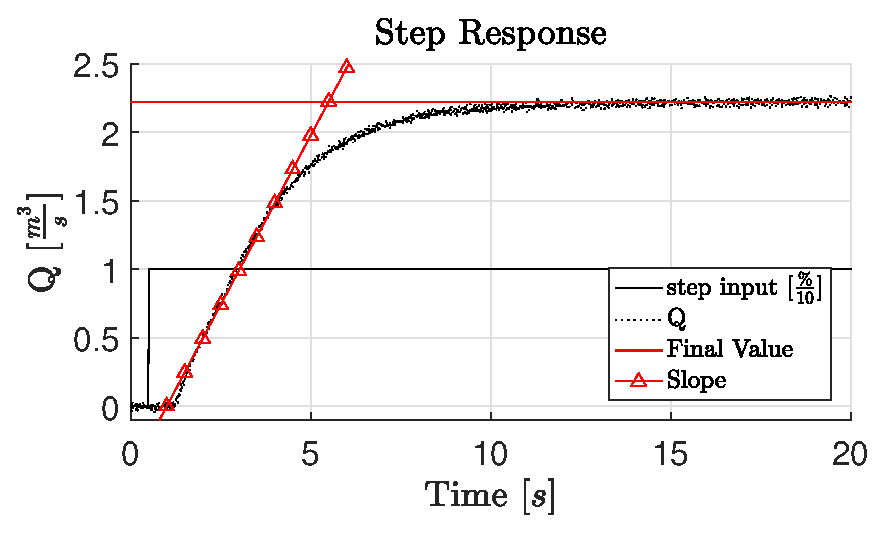
\includegraphics[width=\textwidth]{figures/04ExperimentsAndLabWork/StepResponseLabeled.eps}
    \caption{response to a step input with value 10}
	\label{fig:stepin}
\end{figure}
\todo[color=07controllerDesign]{can we make the axis look like they are made by LaTeX as well?}
\\ \\ \\ \\
\todo[color=07controllerDesign]{structure}
\chapter{Controller Implementation}\label{ch:cimplement}
\chapter{Discussion}\label{ch:discussion}
\todo[color=09discussion]{Discussion no text yet}

During the project, our focus shifted. We aimed at developing a control technique, to achieve a constant flow, employing
all three pumps, and using minimal amount of energy. In the end, using control methods taught during our semester, we have
developed a PID Controller, capable of maintaining a certain flow, employing only one pump.

We believe, our initial goal was a high one. However possibly not achievable at our level and with our level of knowledge.
Such goals were previously achieved by researchers present at this university. 

During the project, we have gained a lot of insight into pumps, and were able to apply principles and knowledge
learned during the semester. This has benefited us greatly, since pumps are used in various systems throughout the industry.

Our belief is that, further work can be done on the same setup, in upcoming semesters, aiming at our initial goal and
even setting higher ones. 


\chapter{Conclusion}\label{ch:conclusion}
\todo[color=10conclusion]{Conclusion no text yet}
\chapter{Data Aquisition}\label{ch:dataAq}

\printbibliography[heading=bibintoc]
\label{bib:mybiblio}
\appendix
\end{document}
